\Section{StreamIt Programming Language}
\label{sec:streamit}

StreamIt~\cite{streamitcc} is an architecture independent language
that is designed for stream programming. In StreamIt, programs are
represented as graphs where nodes represent computation and edges
represent FIFO-ordered communication of data over tapes. The language
features several novelties that are essential for large scale program
development. The language is modular, parameterizable, malleable and
architecture independent. In addition, the language exposes the
inherent parallelism and communication patterns that are prevalent in
streaming programs.

\begin{figure*}[t]
  \begin{minipage}[t]{4.0in}
    {
	\begin{scriptsize}
	  \begin{verbatim}
	    int->int filter ZigZagScan(int N, int[N] Order) {
	      work pop N push N {
	        for (int i = 0; i < N; i++) {
	          int pixel = peek(Order[i]);
	          push(pixel);
	        }
	        for (int i = 0; i < N; i++) {
	          pop();
	        }
	      }
	    }
	  \end{verbatim}
	\end{scriptsize}
    }
    % \vspace{-3pt}
    \caption{Example filter implementing zig-zag scanning.}
    % \label{fig:zigzag-filter}
  \end{minipage}
  ~~\vrule~~
  \begin{minipage}[t]{3.0in}
    {  
      % TODO: change to EPS figure with arrows for zig-zag order
	\begin{scriptsize}
	  \begin{verbatim}
	    int[64] Order = 
	      {00, 01, 05, 06, 14, 15, 27, 28,
	       02, 04, 07, 13, 16, 26, 29, 42,
	       03, 08, 12, 17, 25, 30, 41, 43,
	       09, 11, 18, 24, 31, 40, 44, 53,
	       10, 19, 23, 32, 39, 45, 52, 54,
	       20, 22, 33, 38, 46, 51, 55, 60,
	       21, 34, 37, 47, 50, 56, 59, 61,
	       35, 36, 48, 49, 57, 58, 62, 63};



	  \end{verbatim}
	\end{scriptsize}
    }
    % \vspace{-3pt}
    \caption{Example zig-zag order for filter.}
    \label{fig:zigzag-order}
  \end{minipage}
\end{figure*}

\SubSection{Filters as Programmable Units}
In StreamIt, the basic programmable unit is a {\it filter}.  Each
filter has an independent address space; all communication with other
filters is via the input and output channels (and occaisionally via
control messages, see Section~\ref{sec:messaging}).  Filters contain a
work function that represents a steady-state execution step.  The work
function pops (i.e., reads) items from the filter input tape and
pushes (i.e., writes) items to the filter output tape. A filter may
also {\tt peek} at a given index on its input tape without consuming
the item; this makes it simple to represent computation over a sliding
window or to perform permutations on the input stream. The {\tt push},
{\tt pop}, and {\tt peek} rates are declared as part of the work
function, thereby enabling the compiler to apply various optimizations
and construct efficient execution schedules.

A filter is akin to a class in object oriented programming with the
work function serving as the main method. A filter is parameterizable,
and this allows for greater malleability and code reuse. An example
filter is shown in Figure~\ref{fig:zigzag-filter}. This filter
consumes a stream whose elements are of type {\tt int} and produces a
stream of the same type. It implements the zig-zag scanning pattern
used in the run-length encoding of quantized DCT coefficients (see
Figure~\ref{fig:zigzag}). Typically, the zig-zag scan operates on a
8x8 matrix. An instantiation of a filter can specify the matrix
dimensions, as well as the desired ordering. In MPEG, there are two
possible scan orders. The {\tt Order} parameter can define the
specific scan pattern that is desired. For example, to implement the
order shown in Figure~\ref{fig:zigzag}(a), the array is defined as
shown in Figure~\ref{fig:zigzag-order}.

In this example, the DCT matrix is represented as a unidimensional
stream. The filter peeks or inspects the elements and copies them to
the output stream in the specified order. Once all the DCT
coefficients are copies, the input stream is deallocated from the tape
with a series of pops.

\begin{figure}[t]
\begin{center}
%\vspace{-24pt}
% \framebox{
 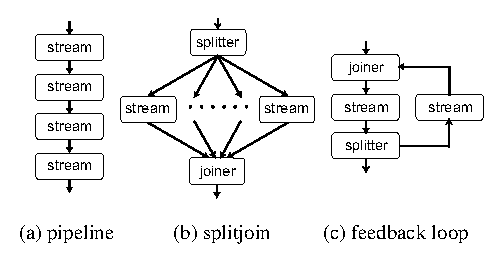
\includegraphics[scale=1, angle=0]{./constructs-eg.eps}
%}
% \vspace{-6pt}
% \nocaptionrule
 \caption{Hierarchical streams in StreamIt.}
 \label{fig:containers}
\end{center}
\end{figure}

\SubSection{Hierarchical Streams}
In StreamIt, the application developer focuses on the hierarchical
assembly of the stream graph and its communication topology, rather
than on the  explicit management of the data buffers between filters.
StreamIt provides three hierarchical structures for composing filters
into larger stream graphs (see Figure~\ref{fig:containers}).

\paragraph{Pipeline.}
The {\it pipeline} stream construct composes streams in sequence, with
the output of one connected to the input of the next.  An example of a
pipeline appears in Figure~\ref{fig:decoder-pipeline}. A pipeline is a
single input to single output stream. The decoding pipeline in the
figure consists of three streams. The first is a filter which zig-zag
unorders the input stream, and prepares the data for the inverse
quantization and DCT. The output of the filter is consumed by a stream
named {\tt IQ} which is a pipeline itself (not shown). This example
illustrates the hierarchical nature of stream composition in
StreamIt. The {\tt IQ} pipeline performs the inverse quantization, and
produces an output stream that is in turn consumed by another stream
which performs the inverse DCT. As in the case of a filter, pipelines
are also parameterizable.

\begin{figure*}[t]
  \begin{scriptsize}
    \begin{verbatim}
	int->int pipeline Decode()
	{ 
	  int Order[64] = {...};     // initialized as shown earlier
	  add ZigZagScan(64, Order);
	  add IQ();                  // inverse quantization
	  add IDCT(8, 8);            // inverse DCT (8x8 matrix)
	}
    \end{verbatim}
  \end{scriptsize}
  % \vspace{-3pt}
  \caption{Example MPEG decoder pipeline.}
  \label{fig:decoder-pipeline}
\end{figure*}

The {\tt add} keyword in StreamIt constructs the specified stream
using the input parameters. The {\tt add} statement may only appear in
non-filter streams.  In essence, filters are the leaves in the
hierarchical construction, and composite nodes in the stream graph
define the encapsulating containers. This allows for modular design
and development of large applications, thereby  promoting
collaboration, increasing code reuse, and simplifying debugging.

\paragraph{Split-Join.}
The {\it splitjoin} stream construct distributes data to a set of
parallel streams, which are then joined together in a roundrobin
fashion. In a splitjoin, the {\it splitter} performs the data
scattering, and the {\it joiner} performs the gathering. A splitter is
a specialized filter with a single input and multiple output
channels. On  every execution step, it can distribute its output to
any one of its children in either a {\it duplicate} or a {\it
roundrobin} manner. For the former, incoming data are replicated to
every sibling connected to the splitter. For the latter, data are
scattered in a roundrobin manner, with each item sent to exactly one
child stream, in order. The splitter type and the weights for
distributing data to child streams are declared as part of the syntax
(e.g., \texttt{split duplicate} or \texttt{split
roundrobin($w_1,\ldots,w_n$)}). The splitter counterpart is the
joiner. It is a specialized filter with  multiple input channels but
only one output channel. The joiner gathers data from its predecessors
in a roundrobin manner (declared as part of the syntax) to produce a
single output stream.

\begin{figure*}[t]
  \begin{scriptsize}
    \begin{verbatim}
	// N = macroblock size + motion vector data size;
	// W = picture width (resolution in pixels);
	// H = picture width (resolution in pixels);

	int->int splitjoin YCrCbDecoding(int N, int W, int H)
	{
	  // 4:2:0 chroma format
	  split roundrobin(4*N, 1*N, 1*N);

	  // last two parameters indicate necessary upsampling in x-y directions
	  add LuminanceChannel  (W, H, 0, 0);
	  add ChrominanceChannel(W, H, 2, 2);
	  add ChrominanceChannel(W, H, 2, 2);

	  join roundrobin(1, 1, 1);  
	}
    \end{verbatim}
    % TODO: validate 4*N, N, N parameters to above streams
  \end{scriptsize}
  % \vspace{-3pt}
  \caption{Example MPEG decoder splitjoin.}
  \label{fig:decoder-sj}
\end{figure*}

The splitjoin stream is a convenient and natural way to represent
parallel computation. For example, when the decoder performs the
luminance and chrominance channel processing, the computation can
occur in parallel. In StreamIt, this is expressed as shown in
Figure~\ref{fig:decoder-sj}. The input stream contains the
macroblock data along with the parsed motion vectors. The data is
partitioned and passed to one of three decoding channels, with $4N$
items assigned to the first stream, $N$ items to the second, and $N$
items to the third. The three streams reconstruct the original
pictures with respect to the different color channels, and their
output is combined by the joiner to produce the final decoded picture.

\paragraph{Feedback Loop.}
StreamIt also provides a {\it feedback loop} construct for introducing
cycles in the graph. This stream construct is not used in the decoder,
but may be used in the MPEG encoder.

\SubSection{Teleport Messaging}
\label{sec:messaging}
%%% XXX largely copied from ppopp paper
A notoriously difficult aspect of stream programming, from both a
performance and programmability standpoint, is reconciling regular
streaming dataflow with irregular control messages.  While the
high-bandwidth flow of data is very predictable, realistic
applications such as MPEG also include unpredictable, low-bandwidth
control messages for adjusting system parameters (e.g., desired
precision in quantization, type of picture, resolution, etc.).

For example, the inverse quantization step in the decoder uses a
lookup table that provide the inverse quantization scaling factors.
However, the particular scaling factor is determined by the stream
parser. Since the parsing and inverse quantization tasks are logically
decoupled, any pertinent information that the parser discovers must be
teleported to the appropriate streams.  In StreamIt, such
communication is conveniently accomplished using teleport
messaging~\cite{thies05ppopp}.

\begin{figure*}[t]
  \begin{scriptsize}
    \begin{verbatim}
	01 void->void MPEGDecoder {
	02   ...
	03   portal<InverseDCQuantizer> p;
	04   ...
	05   add Parser(p);
	06   ...
	07   add InverDCQuantizer() to p;
	08   ...
	09 }
	 
	 
	10 int->int filter Parser(portal<InverseDCQuantizer> p) {
	11   work push * {
	12     int precision;
	13     ...
	14     if (...) {
	15       precision = pop();
	16       p.setPrecision(precision) [0:0];
	17     }
	18     ...
	19   }
	20 }

	21 int->int filter InverseDCQuantizer() {
	22   int[4] scalingFactor = {8, 4, 2, 1};
	23   int    precision = 0;

	24   work pop 1 push 1 {
	25     push(scalingFactor[precision] * pop());
	26   }

	27   handler setPrecision(int new_precision) {
	28     precision = new_precision;
	29   }
	30  }
    \end{verbatim}
  \end{scriptsize}
  % \vspace{-3pt}
  \caption{MPEG messaging example.}
  % TODO: add picture
  \label{fig:messaging}
\end{figure*}

The idea behind teleport messaging is for the {\tt Parser} to change
the quantization precision via an asynchronous method call, where
method invocations in the target are timed relative to the flow of
data in the stream (i.e., macroblocks). As shown in
Figure~\ref{fig:messaging}, the {\tt InverseDCQuantizaer} declares a
message handler that adjusts its precision (lines 27-29). The {\tt
Parser} calls this handler through a {\it portal} (line 16), which
provides a clean interface for messaging.  The handler invocation
includes a range of latencies {\tt [min:max]} specifying when the
message should be delivered with respect to the data produced by
sender.

The interesting aspects of teleport messaging are the semantics for
the message latency.  Intuitively, the message semantics can be
thought of in terms of attaching tags to data items.  If the {\tt
Parser} sends a message to a downstream filter with a latency $k$,
then conceptually, the filter tags the items that it outputs in $k$
iterations of its work function. If $k=0$, the data produced in the
current execution of the work function is tagged. The tags propagate
through the stream graph; whenever a filter inputs an item that is
tagged, all of its subsequent outputs are also tagged with the same
message. The message flows through the graph until the tagged data
reaches its intended receiver, at which time, the message handler is
invoked immediately before the execution of the work function in the
receiver.  In this sense, the message has the semantics of traveling
``with the data'' through the stream graph, even though it is not
necessarily implemented this way.  The intuition for upstream messages
is similar.

Teleport messaging exposes the true information flow, and avoids the
muddling of data streams with control-relevant information. Teleport
messaging thus separates the concerns of the programmer from that a
system implementation, thereby allowing the compiler to deliver the
message in the most efficient way for a given architecture. Teleport
messaging also offers other powerful control over timing and latency
beyond what is used in this example~\cite{thies05ppopp}.
